\documentclass{beamer}

\usepackage[french]{babel}
\usepackage[utf8]{inputenc}
\usepackage{graphicx}
\usepackage{phaistos}
\usepackage{movie15}
\usepackage{marvosym}
\graphicspath{ {images/} }
\usetheme{AnnArbor}
\newcommand*\commu{
\includegraphics[height=3.0mm]{communism.png}}
\newcommand*\burger{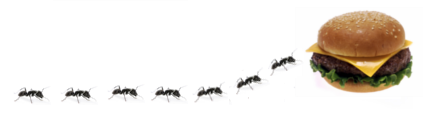
\includegraphics[height=11.8mm,width=42.3mm]{intro.png}}
\title{Simulation du comportement des fourmis: phénomène d'émergence }
\author{  Cardini Yannick  et Caillat-Grenier Geoffroy \commu }
%\author{  Cardini Yannick  et Caillat-Grenier Geoffroy }
\date{Jeudi 26 Avril, 2018}
\institute{Université de Nice Sophia Antipolis \\ Valrose}
\logo{ 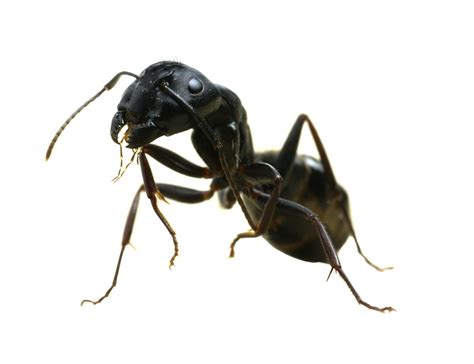
\includegraphics[height=7.0mm]{ant.png}}


\begin{document}
%1ere page
	\begin{frame}
		\titlepage
	\end{frame}
	
%2eme page
	\begin{frame}
	\frametitle{\centerline{\textbf{Introduction} }}
		\begin{itemize}
			\item \Large Le phénomène d'émergence
			\item \Large Procédé pour l'engendrer

		\end{itemize}
		% in preamble
			%aphics[scale=0.9]{intro.png}
			
	\end{frame}
	

	
%4eme page
	\begin{frame}
		\frametitle{\centerline{\textbf{Problématique}}}

				\huge Des règles simples peuvent-elles permettre la création de chemins?

	\end{frame}
		
	\begin{frame}
	\frametitle{\centerline{\textbf{Le modéle netlogo}}}
		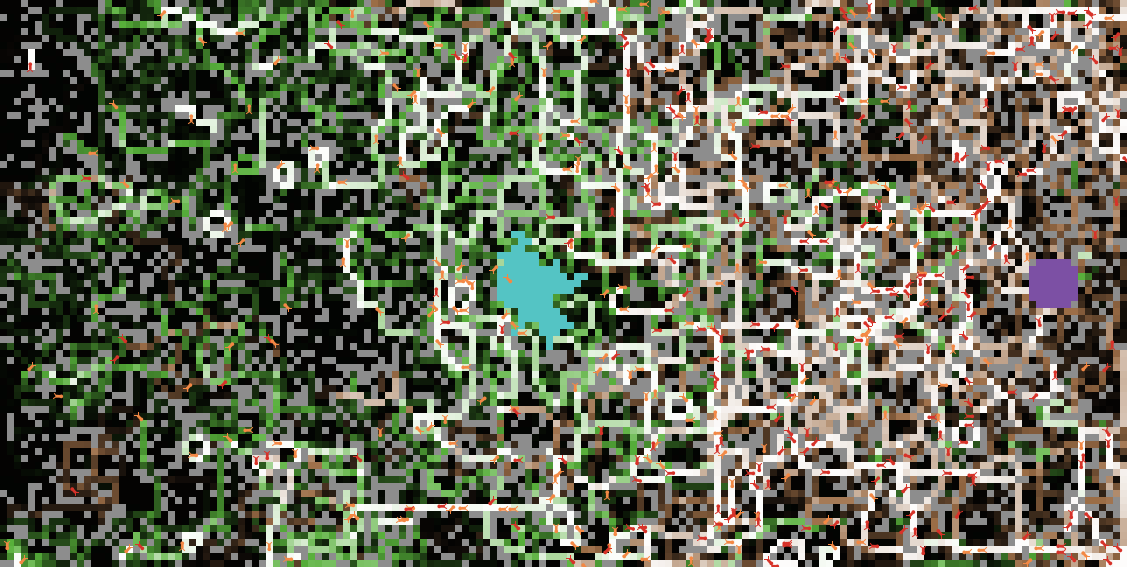
\includegraphics[width=\textwidth,height=\textheight,keepaspectratio]{netlogo.png}
	\end{frame}

%5eme page
	\begin{frame}
	\frametitle{\centerline{\textbf{La modélisation}}}

			\begin{enumerate}
				\item \Large Hypothèses simplificatrices \pause
				\item \Large Description du modèle\pause
				\item \Large Cadre expérimental \pause
				\item \Large Protocole expérimental
			\end{enumerate}

	\end{frame}
	


%6eme page
	\begin{frame}
	\frametitle{\centerline{\textbf{Résultats} }}
		\begin{figure}
	 		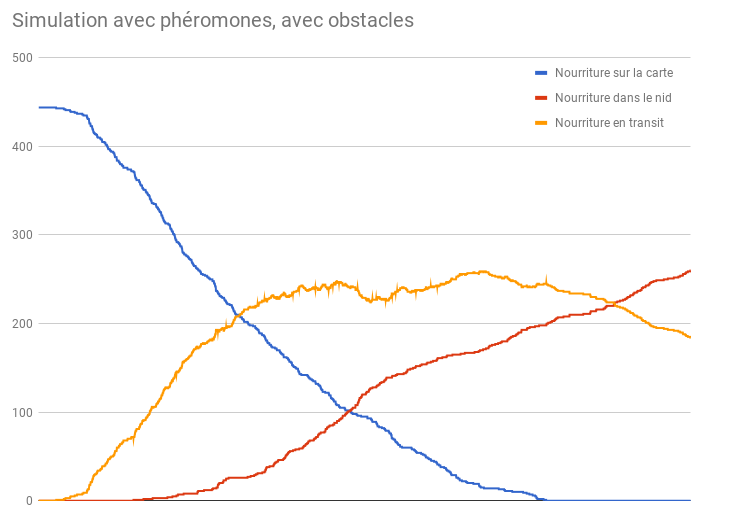
\includegraphics[height = 6.0cm]{phe_obs.png}
	 		\caption{Résultat de la simulation avec phéromones et obstacles}
		\end{figure}
	\end{frame}
	
%7eme page
	\begin{frame}
	\frametitle{\centerline{\textbf{Conclusion} }}
		\begin{enumerate}
		\item \Large Conclusion	
			\begin{enumerate}
				\item \Large Emergence d'un comportement complexe \pause
				\item \Large Une réalité difficile à simuler
			\end{enumerate}
		\end{enumerate}
	\end{frame}
\end{document}